% !TEX root = ../main.tex

% 中英标题:\chapter{中文标题}[英文标题]
\chapter{绪论}[Introduction]

\section{课题研究的背景和意义}[Background, objective and significance of the subject]

% 正文内容,注意LaTeX分段有两种方法,直接空一行或者使用<\par>
% 默认首行缩进,不需要在代码编辑区手动敲空格
地球上的一切都是信号的来源。人类不断测量和收集自然界发生的信号,如温度、风速、降雨量和太阳黑子强度,以适应环境。此外,几十年来,各种各样的工业活动已经在大多数行业领域产生了大量的数据,例如商业(如销售和市场趋势)、金融(如股票价格)、生物医学(如心脏和大脑活动)和制造业(如产量)。在每个行业领域,数据所有者都积极地收集和利用它们来改进产品、流程和服务。特别是,随着工业 4.0 的出现,工业界已经开始密集地利用大量的传感器来同时监测他们的设施和系统,从而提高了效率、安全性和安全性\cite{yellow1}。

在各种数据类型中,时间序列数据在医学、气象学和经济学等学术界已经研究了很长一段时间,现在已经成为大多数实际应用中必不可少的分析对象。时间序列分析是指从时间序列数据中提取有意义的知识的一系列任务,提取的知识不仅可以用来诊断过去的行为,还可以用来预测未来。广为人知的时间序列分析例子包括分类、聚类、预测和异常检测。

随着异常检测收到国内外诸多学者的广泛关注\cite{none5, none4, none3, none2, none1},多元时间序列异常检测领域几个挑战还没有被很好的解决:

异常检测召回率低: 由于异常非常罕见且不均匀,因此很难识别所有的异常。许多正常的实例被错误地报告为异常,而真正复杂的异常被忽略。虽然多年来已经引入了大量的异常检测方法,但是目前最先进的方法,特别是无监督方法(例如\cite{orange17,orange84}) ,仍然经常在现实世界的数据集上引起高度的假阳性\cite{orange20,orange115}。如何减少误报和提高检测召回率是最重要也是最困难的挑战之一,特别是对于不能发现异常的巨大代价。

对高维或非独立数据的异常检测:异常在低维空间中往往表现出明显的异常特征,而在高维空间中则变得隐蔽和不易察觉。高维异常检测一直是一个长期存在的问题。在由一小部分原始特征或自定义特征的简化低维空间中执行异常检测是一个直接的解决方案,例如基于子空间的\cite{orange70,orange77,orange84,orange123}和基于特征选择的方法\cite{orange12,orange109,orange111}。但是,识别复杂的特征(例如,高阶,非线性和异质)相互作用和耦合\cite{orange22}可能在高维数据中是必不可少的,但对于异常检测而言,这仍然是一个主要的挑战。此外,如何保证新的特征空间为特定的检测方法保留适当的信息对于下游的精确异常检测是至关重要的,但是由于上述的未知和异常的不均匀性,这是具有挑战性的。
 
对包含缺失值的多元时间序列进行异常检测:在真实世界中,往往会因为各种非人为因素而导致数据采集不全。例如:传输条件的限制,传感器的自然损坏而没有被及时更换等等而导致数据并数据产生缺失。目前并没有方法在包含缺失值的场景下对时间序列进行异常检测。

\section{国内外研究现状}[Developmental of gas-lubricated bearing and correlated theories]

时序数据的异常检测是数据分析中常见的研究课题,具有重要研究意义和应用价值。目前,研究人员已提出许多异常检测方法\cite{green10,green11,green12} 。

有监督的检测方法需利用带有标签的数据进行训练,学习出输入数据到输出结 果之间的映射关系,待检数据根据该映射关系即可判断出是否为异常,从而将异常检测问题转化为分类问题\cite{green13,green14} 。许多检测方法利用二分类器将时间序列中的所有数 据点划分为两类,表现出正常状态的数据点统一归为一类,即正常数据,将其他数据点归为另一类,即异常数据。常用的二分类器有支持向量机\cite{green15} ,其本质是寻找一 个能够区分正常数据和异常数据的超平面, 并且使该平面距离这两类数据的间隔最 大化以更精准地判别异常 。不同于基于二分类器的检测方法,大多基于多分类器的检测方法借助决策树\cite{green16} 模型将数据点划分为多个类别,从而区分正常数据和异常数据。

时序数据中异常数据量往往远少于正常数据量, 导致明显的标签数量不均衡的 问题,且在许多实际应用中,数据不带有标签。因此, 有监督的检测方法缺乏一定 的灵活性。由于无监督的检测方法不依赖于数据标签即可检测异常,所以无监督方法比有监督方法的运用范围更广、灵活性更强\cite{green10} 。本文主要针对无监督的异常检测方法展开研究。

在无监督的异常检测方法中,一种较为直接的检测思路是通过定义时序数据的正常模式来对比待检数据与正常模式之间的差异,进而检测时序异常 。由于时序数据随时间变化,其分布规律难以捕捉,且普遍存在噪声的干扰,所以通常很难给出正常数据模式的定义, 这加大了时序数据异常检测的难度\cite{green18} 。因此,许多方法计算数据之间的邻近度或重构误差以实现异常检测 。其检测结果不依赖于正常的数据模式,在一定程度上降低了方法的检测难度 。无监督的检测方法包含传统的基于邻近 度的异常检测方法和基于深度学习的异常检测方法。本文主要就这两类介绍其相关成果及目前存在的问题。

\subsection{多元时间序列异常检测的经典方法}

当前,经典方法包括基于线性模型的方法\cite{yellow3} ,基于距离的方法\cite{yellow4} ,基于密度的方法\cite{yellow1}和支持向量机\cite{yellow6} ,仍然是一个可行的算法选择。然而,随着目标系统变得越来越大和越来越复杂,这些方法面临着局限性,即无法操作多维数据或解决标记异常的短缺。特别是,检测时间序列数据中的异常是具有挑战性的,因为沿时间轴的观测值之间的顺序和因果关系需要联合考虑。

% \subsubsection{时域频域分析}
时间序列可以通过时域频域分析来的得到时间序列在频度上的特征值,并用于时间序列异常检测。时间序列数据可以在时域中利用测量的阈值的宽度和高度进行分析。另一种简单而有效的方法是应用傅立叶变换家族中的关系来检查频域表示的数据。根据傅里叶定理,任何周期函数,无论多么复杂,都可以表示为周期分量的组合,例如正弦或余弦的和。傅立叶变换家族中的关系是一个从这些组件中恢复功能的过程。离散傅里叶变换是其中一种常用的方法,其形式如下:
\begin{equation}
    X_k=\sum_{t=0}^{T-1} x_t e^{-i 2 \pi k t / T}, \quad k=0, \ldots, T-1
    \end{equation}
其中 $X_k$ 是从给定输入数据变换的 $k$ 次频率值 $x_t$。一旦你把原始的时间序列转换成一个频谱,并按系数进行排序,你就可以通过反转最高频率来获得季节周期。实际上,快速傅里叶变换(FFT)是 DFT 的一个加速版本。

在统计学上,可以针对一段时间内的时间序列通过数学分析得到相关特征值,通过比较特征值来完成时间序列异常检测。为了对时间序列数据进行数学分析,可以通过计算统计指标(如均值、方差、中位数、分位数、峭度、偏度等)来生成统计模型。使用生成的模型,可以检查新添加的时间序列数据,以确定它是否属于正常边界。

% \subsubsection{基于距离的方法}
许多算法使用两个时间序列之间的显式距离来量化两个时间序列之间的相似性。基于所获得的相似度量,如果新获得的序列与正常序列的距离超出了预期的范围,那么它们将被标记为异常。最常见的距离度量是欧几里得度量,如下公式所示,它将距离计算为连接两个点的一段的长度。
\begin{equation}
    D(\mathbf{x}, \mathbf{y})=\sqrt{\sum_{t=1}^T\left(x_i-y_i\right)^2} .
    \end{equation}
动态时间规整(Dynamic Time Warping)是一种流行的距离测量方法,允许两个序列之间的非线性对齐,这两个序列是局部不相位的[79]。假设有两个序列 $X$ 和 $Y$,它们的长度分别是 $M$ 和 $N$。   
两个序列之间的 DTW 距离计算可以通过:使用动态编程创建成本矩阵 $C$
    \begin{equation}
        C(i, j)=D(i, j)+\min \left\{\begin{array}{l}
        C(i-1, j-1) \\
        C(i-1, j) \\
        C(i, j-1),
        \end{array}\right.
        \end{equation}
    最后,使用$W$计算最终的距离
\begin{equation}
    \operatorname{Dist}(W)=\sum_{k=1}^{k=L} w_k
    \end{equation}
    其中 $i$ 是 $X$ 的数据点,$j$ 是 $Y$的数据点,$D(i, j)$是 $i$ 和 $j$ 之间的距离,而 $C(i, j)$ 是两个序列的最小规整距离。从 $C_{M, N}$到 $C_{1,1}$ 回溯得到最优的规整路径 $W(w_1, w2, ... , w_L)$ ,选择前面的最小累积距离点。最后,使用$W$计算最终的距离
    \begin{equation}
        \operatorname{Dist}(W)=\sum_{k=1}^{k=L} w_k
        \end{equation}
% \subsubsection{基于预测的方法}
此外,也可通过预测模型对时间序列进行异常检测。预测模型是根据过去和现在的状态来预测未来的状态。可以根据预测值与实际值偏差的严重程度来推断异常。例如,ARIMA模型(ARIMA)[80]经常被用来预测时间序列。ARIMA 模型由三部分组成:自回归(AR)模型由滞后值的加权和组成,因此可以将随机变量 $X$ 在时间步长 $t$ 的值建模。
    \begin{equation}
        \operatorname{AR}(p): X_t=\phi_1 X_{t-1}+\phi_2 X_{t-2}+\ldots+\phi_p X_{t-p}+\epsilon_t    
    \end{equation}
其中${\phi}^{p}_{i=1}$ 是自相关系数, $\epsilon$是白噪声, $p$是AR模型的阶数。移动平均(MA)模型计算滞后预测误差的加权和,公式为
    \begin{equation}
        \operatorname{MA}(q): X_t=\epsilon_t-\theta_1 \epsilon_{t-1}-\theta_2 \epsilon_{t-2}-\ldots-\theta_q \epsilon_{t-q}    
    \end{equation}
其中${\phi}^{1}_{i=1}$为移动平均系数,$t$ 表示时间步长$t$ 的模型预测误差,$q$ 为 MA 模型的阶。集成(I)表示使用差异的时间序列,因此在时间步长 $t$ 的数据点是$\hat{X}_t=X_t-X_{t-1}$,当 $d = 1$。中 $d$ 表示差异的顺序。
因此,带有参数的 ARIMA 模型表述如下:
\begin{equation}
    \begin{aligned}
    & \hat{y}_t=\mu+\underbrace{\phi_1 y_{t-1}+\phi_2 y_{t-2}+\ldots+\phi_p y_{t-p}}_{\mathrm{AR}(p)} \\
    & \underbrace{-\theta_1 \epsilon_{t-1}-\theta_2 \epsilon_{t-2}-\ldots-\theta_q \epsilon_{t-q}}_{\text {MA }(q)}, \\
    &
    \end{aligned}
    \end{equation}
其中 $\mu$ 是常数,当 $d = 1$时,$y_t = Y_t-Y_{t-1}$。如1-7所述,在特定时间步骤的每个值都受到以前的观测和预测误差的影响,因此 ARIMA 模拟了时间序列的时间性。同时,差分过程使得时间序列保持平稳,使得 ARIMA 对非平稳时间序列有效。如果时间序列数据具有季节或周期变化,可以使用季节 ARIMA (SARIMA)\cite{sarima}模型。在本例中,我们引入了额外的参数: $P$、 $D$ 和 $Q$,它们处理季节性。这些参数的使用方式与 $p$、 $d$ 和 $q$ 相同。
从根本上说,ARIMA 不能建模多元数据。相反,ARIMA模型外生(ARIMAX)\cite{arimax}模型有一个额外的解释变量或向量自回归模型(VAR)\cite{var}模型使用向量来适应多变量项被用来取代 ARIMA。

% \subsubsection{基于聚类的方法}
在无监督环境下,基于聚类的方法是对数据进行分组和检测异常的简单而有效的选择。一旦您时间序列数据映射到一个多维空间中,聚类算法就会根据它们的相似性将它们按照每个类的重心进行分组。如果新接收的数据样本远离预定义的类中心或者属于任何类中心的概率较低,则模型将它们归类为异常。

流行的数据聚类方法包括 k 均值算法\cite{yellow84} ,一类支持向量机(OCSVM)\cite{yellow85},高斯混合模型(GMM)\cite{yellow88}和基于密度的噪声的空间聚类(DBSCAN)\cite{yellow87}。当数据集具有混合属性(如数值和分类值)时,上述方法可能不足以应用。为了解决这个问题,相关学者提出了 k-均值算法和 k-模式算法的简单结合,既k-原型算法\cite{yellow88}。k-原型算法测量了两个混合型对象$X$和$Y$之间的相似性, 这些对象$X$和$Y$可以通过属性 $A^{r}_{1}, A^{r}_{2}, ... , A^{r}_{p}, A^{r}_{p+1} ,..., A^{c}_{m}$被描述。$X$, $Y$之间的差异可以通过公式表示: 
\begin{equation}
    d_2(X, Y)=\underbrace{\sum_{j=1}^p\left(x_j-y_j\right)^2}_{\text {numeric attributes }}+\underbrace{\gamma \sum_{j=p+1}^m \delta\left(x_j, y_j\right)}_{\text {categorical attributes }}
    \end{equation}
第一个术语是数值属性之间的欧几里得度量,第二个术语是分类属性之间的简单匹配差异。

\subsection{多元时间序列异常检测的深度学习方法}

大多数当代最先进的技术采用了某种形式的深神经网络。本文按照其建模思路将其粗略的分成3类.基于RNN的深度学习方法: 此类模型侧重于沿时间轴方向对时间序列数据进行建模基于GNN的深度学习方法: 此类模型侧重于对不同维度间时间序列的关系进行建模,基于GAN的深度学习方法: 此类模型侧重于一段时间内的数据整体分布进行建模。

% LSTM-NDT [20]方法依赖于基于LSTM的深神经网络模型,该模型将输入序列用作训练数据,并且对于每个输入时间戳,预测了下一个时间戳的数据。LSTMS是自动回归神经网络,在顺序数据中学习顺序依赖性,在每个时间戳上的预测都会使用上一个时间戳的输出中的反馈。这项工作还提出了一种非参数动态误差阈值(NDT)策略,以使用误差序列的移动平均值设置异常标记的阈值。但是,作为一个经常性模型,在许多情况下,这种模型的训练速度很慢。此外,LSTM通常在建模长的时间模式时效率低下,尤其是当数据嘈杂时[62]。

% DAGMM [65]方法使用深度自动编码高斯混合模型,以缩小特征空间的尺寸和用于时间建模的经常性网络。这项工作预测了使用高斯人的混合物的输出,其中每个高斯的参数由深神经模型给出。自动编码器将输入数据点压缩到潜在空间中,然后由经常性估计网络使用该数据标记来预测下一个数据点。两个网络的脱钩训练使模型更加强大。但是,它仍然很慢,无法明确利用模式间相关性[14]。 

% Omnianomaly [45]使用随机复发的神经网络(类似于LSTM变量自动编码器[39])和平面化流量来产生重建概率。它还提出了一个调整后的峰值阈值(POT)方法,用于自动异常阈值选择,以优于先前使用的NDT方法。与先前的艺术相比,这项工作导致了巨大的表现飞跃,但以高训练时间为代价。
% 多尺度对流递归编码器码编码器(MSCRED)[60]将输入序列窗口转换为归一化的二维图像,然后将其通过ConvlstM层传递。该方法能够捕获更复杂的模式间相关性和时间信息,但是无法概括为训练数据不足的设置。 

% MAD-GAN [29]使用基于LSTM的GAN模型来使用发电机对时间序列分布进行建模。这项工作不仅使用预测误差,还使用异常得分中的鉴别损失。 

% MTAD-GAT [62]使用图形注意网络对特征和时间相关进行建模,并将其通过轻巧的封闭式驱动器(GRU)网络,该网络有助于检测而没有严重的开销。传统上,注意力操作使用凸组合进行输入压缩,其中使用神经网络确定权重。 GRU是具有较小参数集的LSTM的简化版本,可以在有限的数据设置中进行培训。 

% CAEM [61]使用类似于MSCRED的卷积自动编码内存网络。它通过CNN传递时间序列,双向LSTM处理输出以捕获长期的时间趋势。此类复发性基于神经网络的模型已显示出高维数据集的高计算成本和较低的可伸缩性[4]。

% USAD [4],GDN [14]和OpenGauss [30]等最新作品不使用渴望资源的经常性模型,而仅使用基于注意力的网络体系结构来提高训练速度。

% USAD方法使用带有两个具有对抗性游戏风格训练框架的解码器的自动编码器。这是通过使用简单的自动编码器专注于低开销的首批作品之一,与先前的艺术相比,训练时间可以减少几倍。图形偏差网络(GDN)方法了解数据模式之间的关系图,并使用基于注意力的预测和偏差评分来输出异常得分。
% OpenGauss方法使用基于树的LSTM,该LSTM具有较低的内存和计算足迹,即使使用嘈杂的数据,也可以捕获时间趋势。但是,由于小窗口作为输入以及简单或没有复发模型的使用,最新模型无法有效捕获长期依赖性。
% 最近提出的命中率[19]方法将香草变压器用作编码器 - 模块网络,但仅适用于自然语言日志数据,不适用于通用连续的时间序列数据作为输入。在我们的实验中,我们将Tranad与最先进的方法Merlin,LSTM-NDT,DAGMM,Omnianomaly,MSCRED,MAD-GAN,USAD,USAD,MTADGAT,MTADGAT,CAE-M和GDN进行了比较。这些方法在异常检测和诊断方面表现出了优越性,但在不同时间序列数据集的性能方面相互补充。其中,只有USAD旨在减少培训时间,但在有限的程度上这样做。就像基于重建的先前工作[4、29、45、60、61]一样,我们开发了一个Tranad模型,该模型使用培训数据来学习广泛的趋势,以在测试数据中找到异常。我们特别改善了异常检测和诊断性能,还减少了这项工作中的训练时间。

% \subsubsection{基于RNN的深度学习方法}

LSTM-NDT\cite{lstm-ndt}方法依赖于基于LSTM的深神经网络模型,该模型将输入序列用作训练数据,并且对于每个输入时间戳,预测了下一个时间戳的数据。LSTM-NDT是自动回归神经网络,在顺序数据中学习顺序依赖性,在每个时间戳上的预测都会使用上一个时间戳的输出中的反馈。这项工作还提出了一种非参数动态误差阈值(NDT)策略,以使用误差序列的移动平均值设置异常标记的阈值。但是,作为一个经常性模型,在许多情况下,这种模型的训练速度很慢。此外,LSTM通常在建模长的时间模式时效率低下,尤其是当数据嘈杂时.

Omnianomaly\cite{Omnianomaly}使用随机递归神经网络(类似于LSTM变量自动编码器)和平面化流量来产生重建概率。它还提出了一个调整后的峰值阈值(POT)方法,用于自动异常阈值选择,以优于先前使用的NDT方法。

DAGMM\cite{dagmm}方法使用深度自动编码的高斯混合模型在特征空间进行维度减化,并使用递归网络进行时间建模。这项工作预测一个输出使用混合高斯,其中每个高斯的参数是由一个深入的神经模型。自动编码器将输入数据点压缩到一个潜在空间中,然后由循环估计网络使用该空间来预测下一个数据点。这两个网络的解耦训练允许模型更加健壮; 然而,它仍然是缓慢的,无法明确利用模态间的相关性。

Dai 等人\cite{ganf}与2022年在ICLR会议上发表了GANF模型。GANF采用 RNN 的方法捕捉时间序列沿时间轴变化的趋势,同时引入贝叶斯网络描述不同时间序列之间的关系,最后采用基于标准化流重建的方式进行异常检测,这种方法更侧重于对时间序列沿时间轴方向变化的特征进行建模。
\begin{figure}[htb]
    \centering
    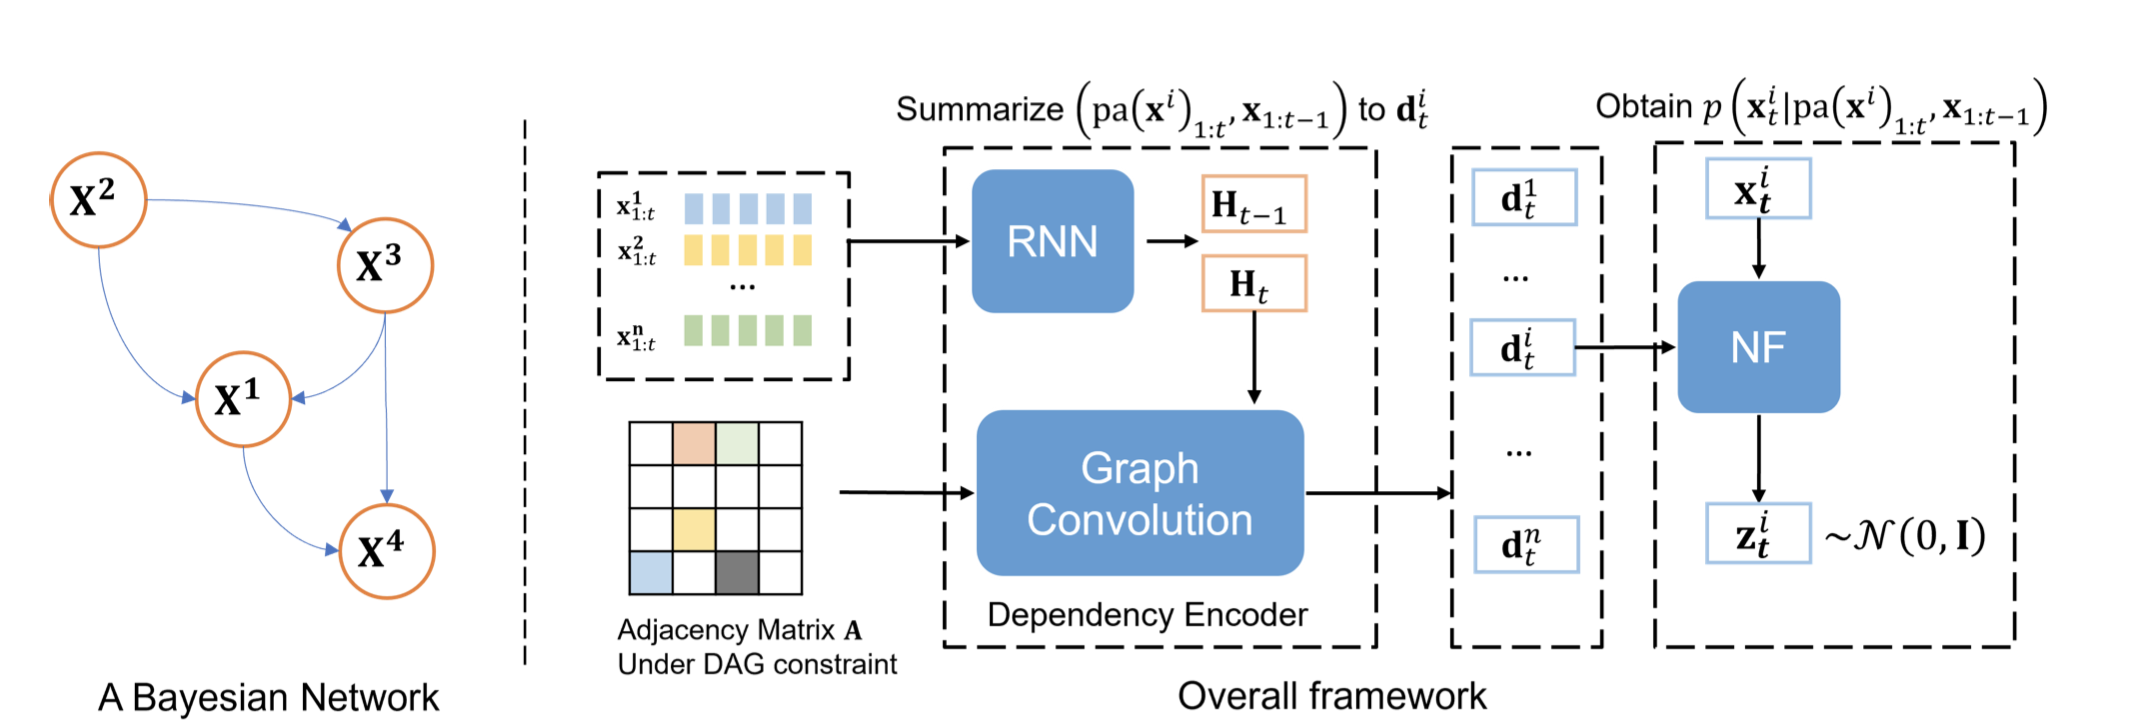
\includegraphics[width = 1\textwidth]{chapter1/GANF.jpg}
    \caption{GANF 模型整体架构\cite{ganf}}
    \end{figure}
如图所示, GANF 使用了一个贝叶斯网络,并通过 RNN 沿着序列维度对$p(\mathcal{X})$ 进行因子分解 然后使用条件规范化流对时间维度进行因子分解。然后,采用一种新的基于图的依赖性编码器来参数化因子分解产生的条件概率。用于因子分解的 DAG 是一个离散的对象,通常很难学习,但是,离散的结构通过一个可微的图形 $\mathbf { a } $反映在依赖编码器中,这个图形的邻接矩阵就是 $\mathbf { a } $。此外,$\mathbf { A } $必须对应于 DAG 的要求可以表示为一个可微方程。因此,可以通过使用基于梯度的优化来联合优化 $\mathbf { A } $和流组件。

% \subsubsection{基于GNN的深度学习方法}
Deng 等人\cite{gdn}于2021年在AAAI会议上发表了GDN模型。GDN采用 GNN 的方法捕捉多个时间序列之间的关联关系,并通过一个全连接层对未来时刻的数据进行预测,以预测值与真实值之间的差异作为异常分数进行异常检测,这种方法更侧重于多元之间序列之间的相关性特征进行建模。
\begin{figure}[ht]
    \centering
    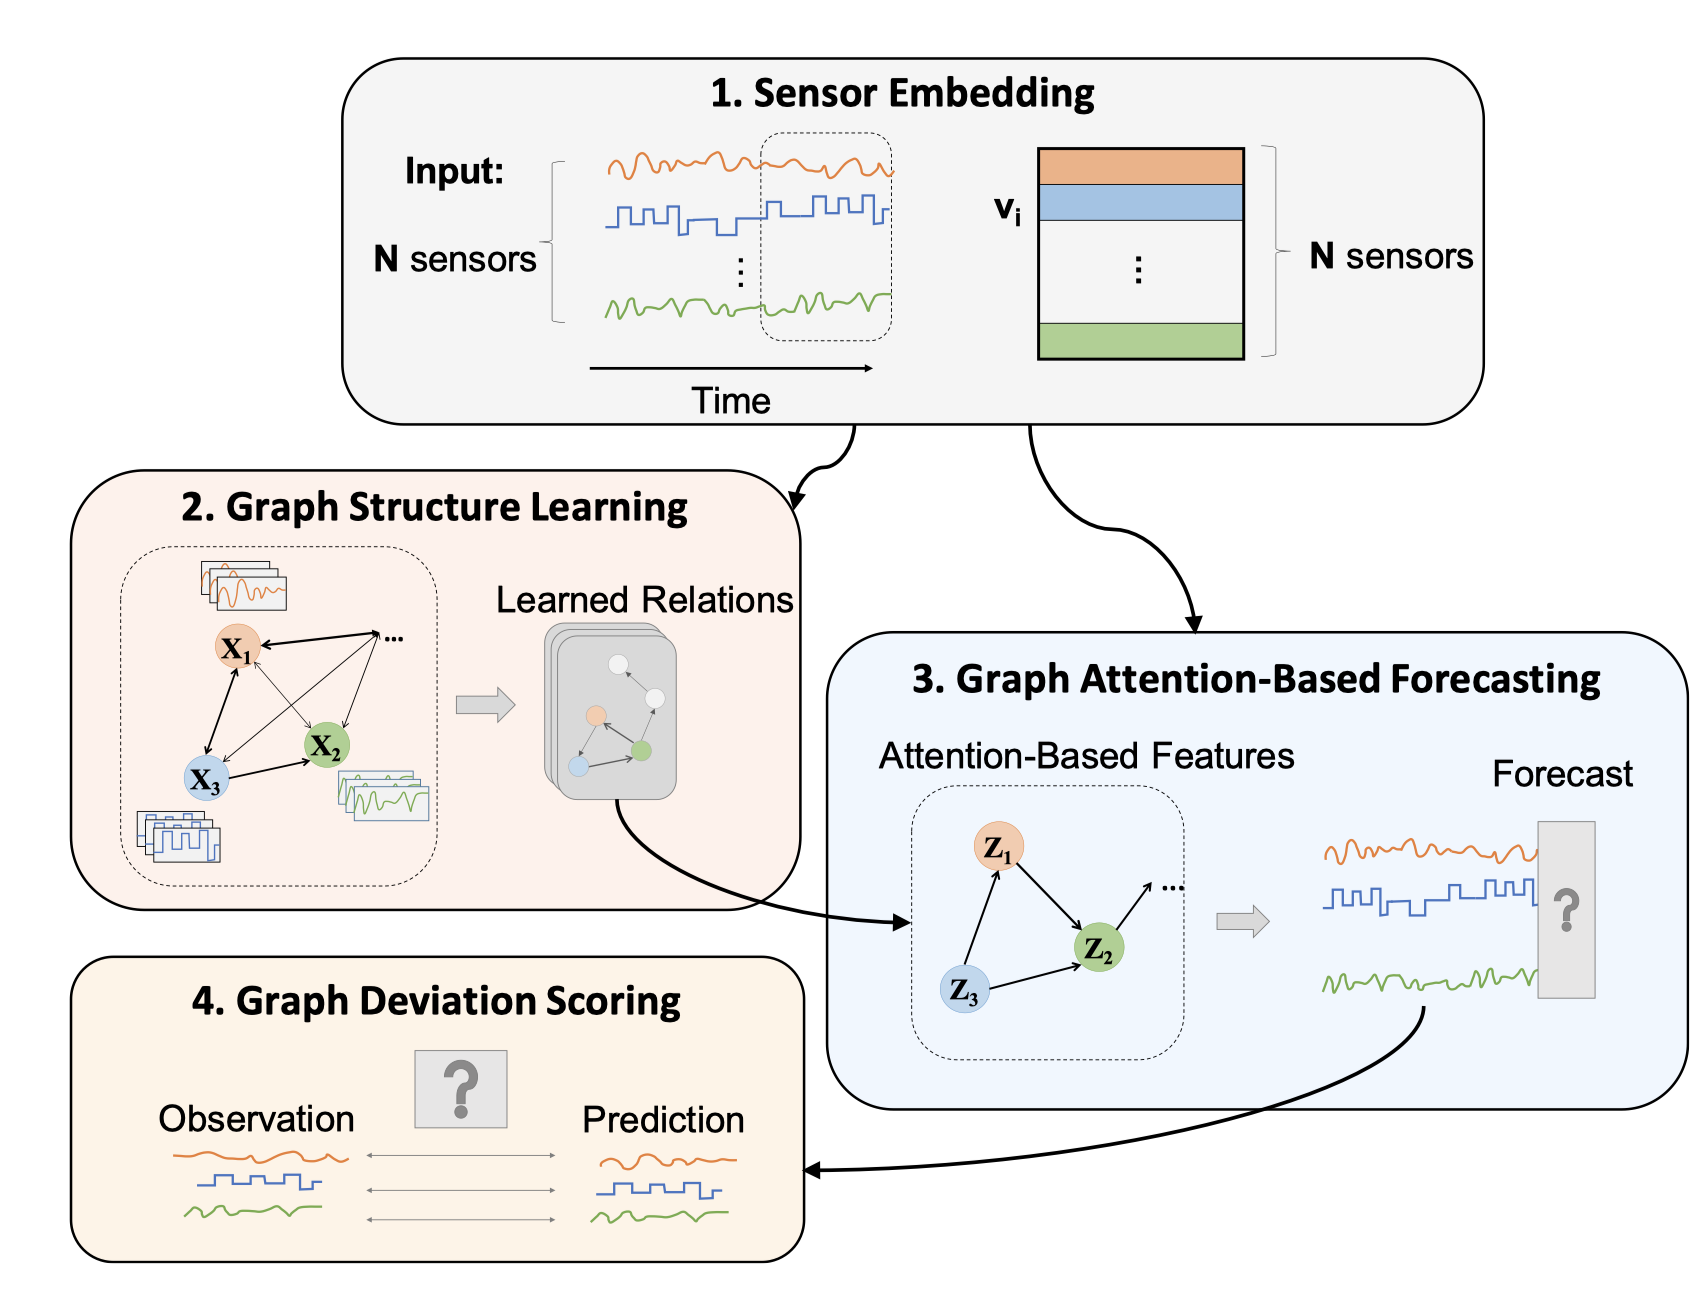
\includegraphics[width = 0.8\textwidth]{chapter1/GDN.jpg}
    \caption{GDN 模型整体架构\cite{gdn}}
    \end{figure}
如图1-2所示,GDN主要包括4个部分,即传感器嵌入, 图结构学习,基于图注意力的预测以及图偏差评分。其中传感器嵌入主要利用嵌入向量捕获每个传感器的独特特性;图结构学习: 学习表示传感器之间依赖关系的图结构;基于图形注意力的预测: 基于图形注意力函数对各传感器的未来值进行预测;图偏差评分: 识别学习关系的偏差,并定位和解释这些偏差。

MTAD-GAT\cite{mtad-gat}使用图形注意网络对特征和时间相关性进行建模,并通过轻量级的门限递归单元(Gated-RecurrentUnit,GRU)网络进行传递,从而在没有严重开销的情况下帮助检测。传统上,注意力操作使用神经网络确定权重的凸组合进行输入压缩。GRU 是 LSTM 的简化版本,参数集较小,可以在有限的数据设置中进行训练。
\begin{figure}[htb]
    \centering
    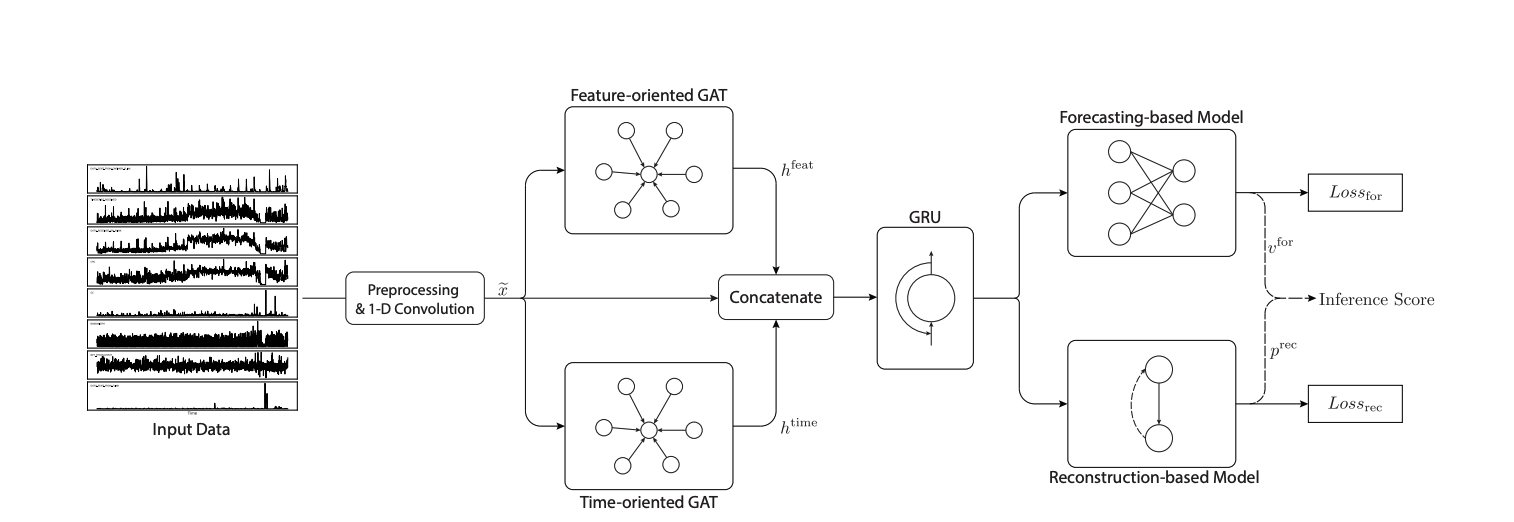
\includegraphics[width = 1\textwidth]{chapter1/MTAD.jpg}
    \caption{MTAD 模型整体架构\cite{mtad-gat}}
    \end{figure}


% \subsubsection{基于GAN的深度学习方法}
Audibert等人\cite{usad}在2020年在KDD上发表了USAD模型。USAD基于自动编码器提出了一种基于对抗性学习的重建方法,该方法通过两个自动编码器对抗性学习重建多元时间序列,并以重建值与真实值之间的差异作为异常分数进行异常检测,这种方法更侧重于对数据的整体分布进行建模。同时Audibert等人提出了训练和检测的两种算法。
\begin{figure}[ht]
    \centering
    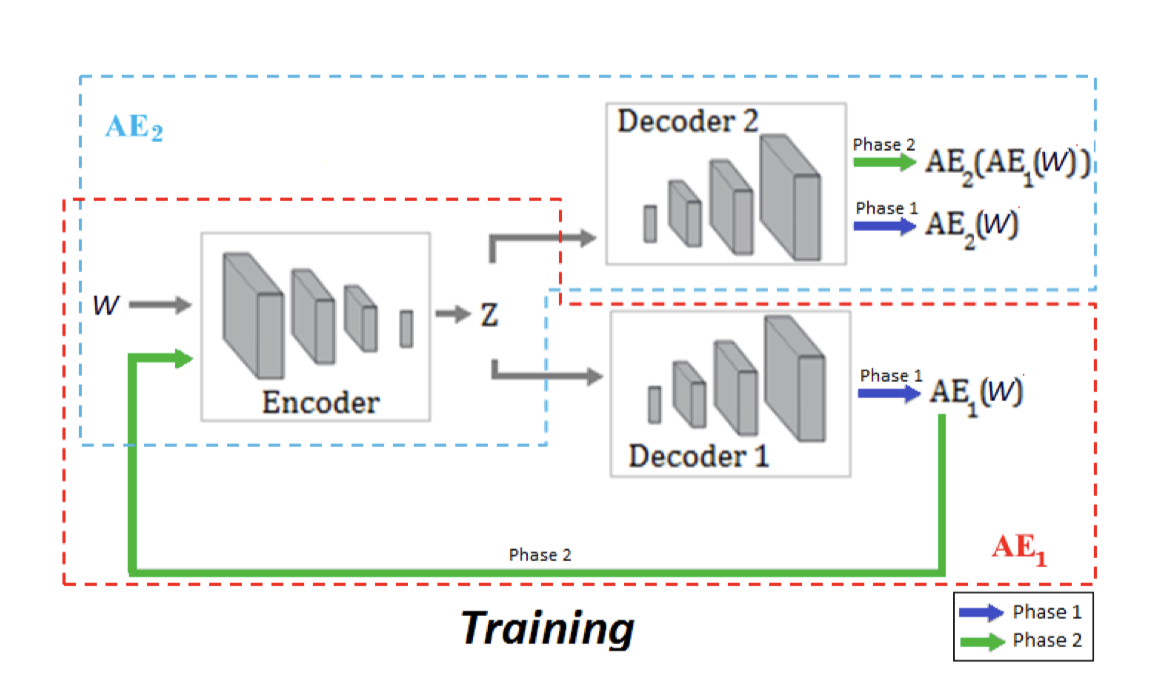
\includegraphics[width = 0.8\textwidth]{chapter1/USAD-TRAINing.jpg}
    \caption{USAD 训练模型架构\cite{usad}}
    \end{figure}
如图1-3所示,USAD模型具有两个自动编码器 AE1和AE2。 在该模型中自动编码器具有双重目的。其中AE1最小化$W$(阶段1)的重建误差,并最小化AE 2(阶段2)的重构输出之间的差异。随着AE1,AE2 最小化了$W$的重建误差(阶段1),它随后最大化了由AE 1(阶段2)重建的输入数据的重建误差。通过这种对抗性学习的方式,使得USAD模型能够更好的学习到时间序列的分布。
\begin{figure}[ht]
    \centering
    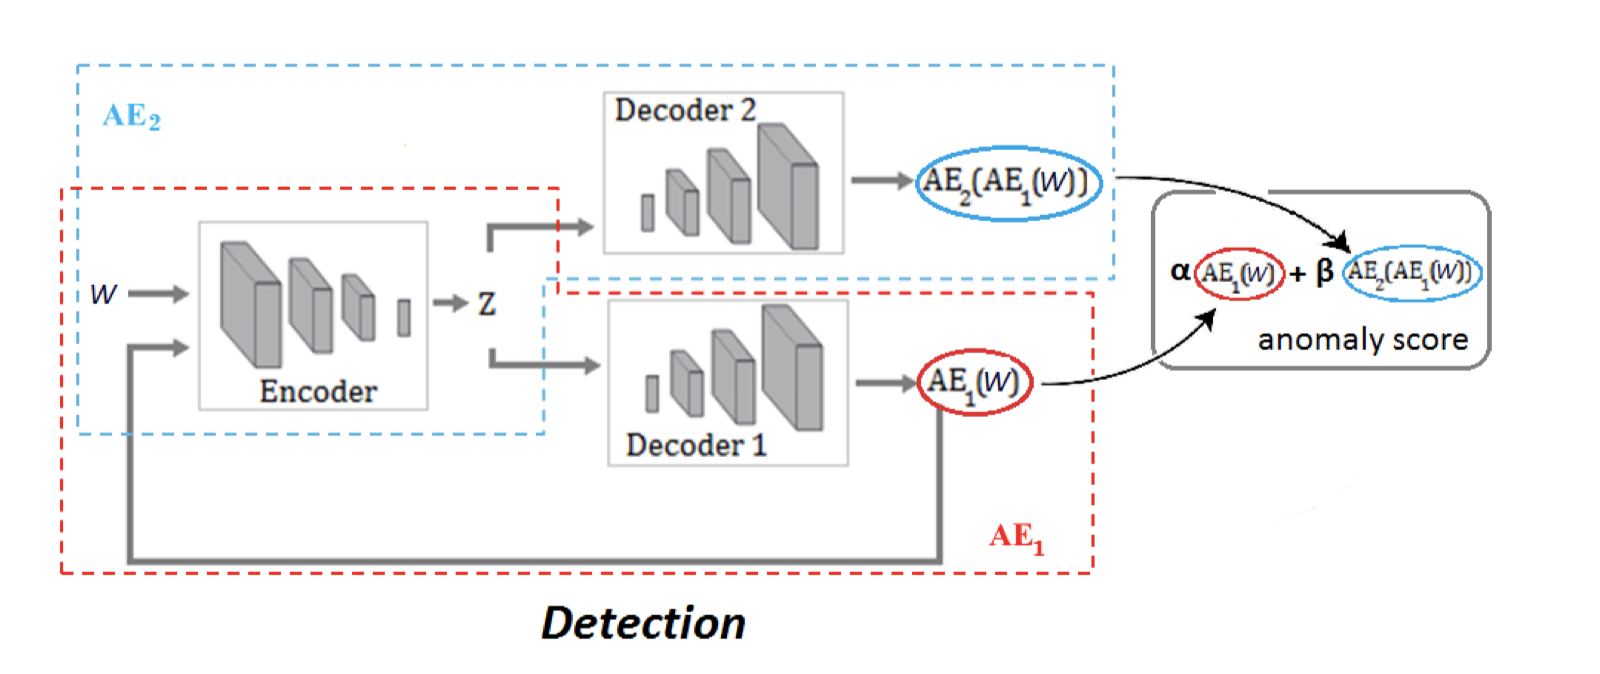
\includegraphics[width = 0.8\textwidth]{chapter1/USAD-DETECTION.jpg}
    \caption{USAD 推断模型架构\cite{usad}}
    \end{figure}
在推断阶段, 时间序列的异常分数通过
\begin{equation}
    \mathscr{A}(\widehat{W})=\alpha\left\|\widehat{W}-A E_1(\widehat{W})\right\|_2+\beta\left\|\widehat{W}-A E_2\left(A E_1(\widehat{W})\right)\right\|_2
    \end{equation}
计算得到,其中$\alpha + \beta = 1$并用于参数化误报和真阳性之间的权衡。如果$\alpha$大于$\beta$,则减少真实阳性的数量并减少误报的数量。相反,如果$\alpha$小于$\beta$,以增加假阳性数量的成本增加了真实阳性的数量。则表示α<βA高检测敏感性方案,而$\alpha > \beta$则表示低检测敏感性。这种参数化方案允许使用单个训练的模型在推断中获得一组不同灵敏度异常得分。

\section{本文的主要研究内容}[Developmental of gas-lubricated bearing]

时间序列异常检测是工业界中一个重要的研究领域。并随着近年来越来越多的行业提倡数字化,智能化,吸引了诸多学者进行研究并提出了非常多的多元时间序列异常检测的算法及模型。然而这些方法都是都是面向完整的时间序列数据进行异常检测任务,然而在真实时间中多元时间序列往往包含着大量的缺失值。例如在工业场景中常常因为数据采集不全,传感器损坏等诸多因素所导致时间序列中包含缺失值。故本文课题为缺失值场景下的多元时间序列异常检测,按照填充-检测和不填充-检测的两种思路对包含缺失值的多元时间序列异常检测任务进行了如下研究:

按照填充-检测的思路,本文首先提出了一种基于对抗生成网络的填充算法,并对填充后的多元时间序列进行异常检测。较好的解决缺失值场景下的多元时间序列异常检测任务。本方法通过与多个基线模型对比,在完整数据集上,本章F1分数超过了第二名的基线0.3\%在缺失30\%数据的场景下F1分数超过了第二名的基线3\%,在缺失50\%数据的场景下F1分数超过了第二名的基线5\%。证明了本文的算法在缺失值场景的有效性。

考虑到在填充-检测的解决方案中,模型在训练时需要同时包含缺失值的时间序列和不包含缺失值的时间序列进行学习。这对数据的要求较高,在现实应用中实现难度较大。填充-检测的思路方案依然不能完美的解决缺失值多元时间序列异常检测问题。故本文提出了一种不填充-检测思路的多元时间序列异常检测方案,其基于注意力机制对缺失值时间序列进行重新表征,将不完整的多元时间序列重新表征为完整的高维表征,进而通过对该表征进行异常检测,更鲁棒的解决缺失值场景下的异常检测任务。本方法在三个常用经典时间序列数据集上进行的实验表明,该方法在缺失值场景下对比传统时间序列异常检测方法效果更好。最后,本文通过消融实验验证了各模块的有效性。

% 本文的主要研究缺失值场景下的多元时间序列异常检测算法,提出了缺失值场景下的多元时间序列异常检测模型 MMAD (Missing Multi Time Series Anomaly Detection),该模型主要结合自注意力机制条件标准化流来完成缺失值场景下的异常检测算法。最后通过在公开数据集上进行实验验证本文提出的有效性。
% \begin{enumerate}
%     \item 缺失值场景下的多元异常检测算法研究
%     提出一种面向缺失值的多元时间序 列的异常检测算法MMAD (Missing Multi Time Series Anomaly Detection),该算法首次提出了一种缺失值场景下的多元时间序列异常检测解决方案。
%     \item 基于掩码注意力机制的缺失值多元时间序列表征算法
%     提出的一种掩码注意力机制模块 (MMAR)将包含缺失值的不完整时间序列数据映射为完整的高维嵌入表征,该表征融合了时间信息、缺失值信息以及观测值信息;
%     \item 基于条件标准化流的标准化分布变换模块(CNF-AD)
%     提出一种基于条件标准化流的标准化分布变换模块(CNF-AD)对该表征进行重建,该模块学习一个可逆变换函数实现一个简单分布(例如高斯分布)与真实分布近似之间的映射,通过该函数与简单分布计算观测值在真实分布中的近似概率,以该概率作为异常分数进行异常检测。
% \end{enumerate}


\section{论文主要结构与安排}[Main research contents of this subject]
本论文的章节划分安排如下: 第一章是绪论,主要介绍本文的研究背景和意义,面临的挑战以及当前主要的两类异常检测算法研究现状, 在绪论最后总结了本文主要的研究内容。

第二章是缺失值时间序列异常检测技术概述。该章节主要介绍时间序列异常检测技术的基本知识,例如时序数据的异常类型,时间序列的基本属性等;同时介绍了本文所利用到的一些关键技术,例如注意力机制和标准化流技术。

第三章按照填充-检测的思路,首先提出了一种基于对抗生成网络的填充算法,并对填充后的多元时间序列进行异常检测。较好的解决缺失值场景下的多元时间序列异常检测任务。随后通过实验证明本文的算法在缺失值场景的有效性。

第四章按照不填充-检测思路,首先提出了一种基于注意力机制对缺失值时间序列进行重新表征,将不完整的多元时间序列重新表征为完整的高维表征,进而通过对该表征进行异常检测的方案,随后在三个常用经典时间序列数据集上进行的实验表明,该方法在缺失值场景下对比传统时间序列异常检测方法效果更好。最后,本文通过消融实验验证了各模块的有效性。